\chapter{Spectral Uplifting} \label{chap:spectralUplifting}

While spectral rendering offers many advantages in terms of physical correctness, it is often neglected and traded off for the RGB color representation due to its ease of use and memory efficiency. Even the physically-based phenomena can be ``faked'', and, therefore, many conventional rendering systems are RGB-based. 

Another reason for the disinclination towards spectral renderers is the deficiency of spectral textures. The process behind their creation is, in comparison to RGB-based textures, a lot more complicated. It usually requires a real-life model whose reflectance spectra must be measured with a spectrometer, which is, in many cases, virtually impossible.  

Spectral renderers are, nonetheless, used both in the research and in the commercial sphere (e.g. ART, Mitsuba, Manuka). To eliminate the need for a repeated creation of the textures from scratch, a technique for utilizing the already existing RGB models by converting them to their spectral variants has been proposed. We refer to this process as \emph{spectral uplifting}, however, other sources also use the term \emph{spectral upsampling}~\cite{sigmoidMethod}.

Converting an RGB value into its respective spectrum poses multiple difficulties. As the relationship between the spectral and the RGB domain is not bijective (specifically, infinitely many spectral distributions render the same RGB values), distinctive approaches to the conversion process may render different spectral distributions. Although all of them might be correct in terms of the resulting RGB value, it is possible that none of them would be identical to spectral distribution measured with a spectrometer.

This does not cause a problem under standard illuminant with regard to which the RGB values were uplifted. However, as already mentioned in~\cref{item:metamerism}, changing the illuminant may result in a rather significant color change due to metamerism. Therefore, our uplifted spectra might behave differently than they would in real world. sem dam obrazok ak ho budem mat

We begin this chapter by reviewing the already existing approaches to spectral uplifting. We then talk about a novel technique, \emph{constrained spectral uplifting}, which provides means for eliminating metamerism during uplifting and the implementation of which is the goal of this thesis.

\section{Uplifting methods} \label{sec:upliftingMethods}

Although there have been multiple attempts at spectral uplifting, not many meet all the conditions required for a successful and complete conversion. Some of the methods, for example, output reflectance spectra with values outside the (0,1) range, others work for saturated colors only, others cause noticeable round-trip errors (i.e. the difference between the original RGB and the RGB of the uplifted spectrum is not negligible), etc.

Following, we overview the most popular approaches to spectral uplifting and call attention to their advantages and disadvantages. We base most of this section on an article by~\citet{upsamplingTechniques}, which, in addition to providing a survey of existing techniques, proposes a new one that is considered to be the current state of the art.

One of the first techniques was proposed in an article by~\citet{upsamplingMacAdam}, which primarily focused on achieving the highest possible brightness for a given color saturation in printing. The uplifting process was only a byproduct of a proof of the limits to the colors' brightness, created especially for representing the reflectance of the researched colors (i.e colors of maximum brightness for any given saturation). Although this method is not limited to a specific input, it produces spectra that are box-shaped and only consist of rising and falling edges. This type of representation is unsuitable for reflectances usually found in nature, which tend to have a smoother curve.

Another technique was proposed by~\citet{upsamplingSmits}. In this case, the uplifting is based on a box basis split into 10 discrete bins, which are derived using an optimization algorithm that accounts for energy conservation and aims for overall smoothness of the spectra. This approach is practically implemented and widely used, as it provides satisfactory results in the sRGB gamut~\cite{upsamplingJakobHanika}. However, in some cases, the uplifted spectra acquire values above 1, which does not satisfy the (0,1) range criterion. Furthermore, round trips consisting of uplifting an RGB value and converting the resulting spectrum back to RGB produce slight color differences, which are only amplified in scenes with multiple reflections. Lastly, this approach becomes unstable when used with wider gamuts, as it was not designed for this purpose.

The goal of the method proposed by~\citet{upsamplingMeng} is wide-gamut uplifting. It also concentrates on optimizing the uplifting algorithm for spectral smoothness. However, it does not take energy conservation into account, which results in images with colors that have no physical counterpart (i.e. no real material could produce such colors). \citet{upsamplingMeng} try to solve this by introducing a set of scaling methods for mapping the uplifted spectra to valid reflectances. These, however, fail upon uplifting bright colors. 

One of the most recent uplifting techniques has been proposed by~\citet{upsamplingOtsu}. It is based on the observation that a typical measured reflectance spectrum can be represented with only a few principle components. The method uses clustered principal component analysis (PCA) and, unlike many other approaches, does not presume that spectra must necessarily be smooth. Such a simplification both eliminates the requirement of having a smoothness heuristic and enables the reconstructed spectra to match the actual measured spectra pretty well. This approach, however, has its downsides. Firstly, the method does not necessarily satisfy the (0,1) range criterion. Therefore, the values must be clamped, which results in color reproduction errors. Moreover, since there is no interpolation across clusters, similar RGB values may produce very different spectra, which might lead to discontinuities in rendering. However, in multiple cases, this method has been shown to outperform all of the already mentioned ones~\cite{upsamplingJakobHanika}.

A large part of this thesis is based on the article by~\citet{upsamplingJakobHanika}, which discusses a parametric function space for efficient representation of spectral reflectance curves and its subsequent utilization in spectral uplifting. We therefore describe their approach in more detail.

The goal was to create a spectral representation that would be both energy-conserving and would have a successful round-trip, i.e. the Delta E difference between the original RGB and the RGB obtained by conversion to spectra and back would be as small as possible. Based on the equation specifying the Delta E error, a simple analytical model has been created. Spectra in accordance with this model are represented as follows:
\begin{equation} \label{sigmoidRepresentation}
f(\lambda)=S(c_{0}\lambda^2+c_{1}\lambda+c_{2}),
\end{equation}
where $f(\lambda)$ is the resulting spectrum, $S$ is a simple sigmoid function and $c_{i}$ are coefficients of a second-order polynomial. Therefore, all spectra in this space are represented by three parameters.

In addition to energy conservation, the resulting spectra do not violate the (0,1) range constraint. They are smooth and simple, similarly to reflectance spectra of real-life surfaces. Another advantage is memory efficiency, as storing one spectrum requires only three values.

However, representing spectra as such also has its drawbacks. For example, there is currently no straightforward, well-defined computation of the RGB $\to$ spectrum conversion in such a domain. One of the possible solutions is to integrate an iterative optimizing process to find a coefficient triplet that would evaluate to the desired RGB.

In this specific implementation, this process is performed by the CERES solver~\cite{ceres-solver}, which requires only an initial guess and a metric according to which it improves the guess (i.e. the Delta E error originating from round-trips). As it requires only a few iterations to converge to 0, the conversion of one RGB triplet is rather fast.

The uplifting process itself works by pre-computing RGB:spectra mappings and storing them in a texture. During rendering, only the required spectra are looked up.

Obviously, it is impossible to store mappings for every RGB triplet --- the RGB space needs to be discretized as efficiently as possible.~\citet{upsamplingJakobHanika} propose a specific discretization method, which divides the sRGB space into three quadrilateral regions in which the coefficients are very smooth. For satisfactory results, only three 3D cubes of size $64^3$ are required.

Another approach is to store all mappings in a table based on a 3D regular grid inside an RGB cube~\cite{upsamplingFluorescence}. As this approach is already used in ART and is very similar to the one in this thesis, we describe the pseudo-algorithm used to create such an uplifting model in~\cref{alg:upliftingAlgSigmoid}.

\begin{algorithm}[t!]
	\caption{Spectral uplifting by~\citet{upsamplingJakobHanika}}
	\label{alg:upliftingAlgSigmoid}
	\begin{algorithmic}[1]
		\State create $RGBCube$ with empty RGB:spectra mappings
		\State $unfittedPoints \gets$ a list of all lattice points in $RGBCube$
		\State $centerPoint \gets$ index of the middle of $RGBCube$
		\Statex \Comment{$RGBCube[centerPoint].rgb \simeq (0.5,0.5,0.5)$}
		\State $centerPoint.coefficients \gets (0,0,0)$
		\Statex \Comment ``guess'' the coefficients at $centerPoint$
		\State run the CERES optimizer for $RGBCube[centerPoint]$
		\State remove $RGBCube[centerPoint]$ from $unfittedPoints$
		\While {$unfittedPoints$ is not empty}
		\ForAll{$point \in unfittedPoints$}
		\If{$point$ has a neighbor $v$ with defined coefficients}
		\State $point.coefficients \gets v.coefficients$
		\State run the CERES optimizer for $point$
		\If{optimization was successfull}
		\State remove $point$ from $unfittedPoints$
		\EndIf
		\EndIf
		\EndFor
		\EndWhile
	\end{algorithmic}
\end{algorithm}

Discretization of the RGB space does not, however, eliminate the need for uplifting RGB values that have no mapping in the spectral uplifting model. In such case, the unknown spectral reflectance values must be computed from the already existing mappings. As the RGB value we wish to uplift falls into a specific voxel in the RGB cube, without much elaboration, three straightforward methods of how to uplift it come to mind:
\begin{enumerate}
	\item weighted interpolation of spectra in voxel corners
	\item weighted interpolation of coefficients in voxel corners
	\item using the coefficients of the nearest voxel corner (\emph{nearest neighbor} approach)
\end{enumerate}

We present the outcomes of these approaches when used for uplifting an RGB texture in~\cref{fig:sigmoidTexture}. We also compare them to the original texture and provide the difference images.

Although the original paper suggests that interpolating coefficients should, within limits, produce reasonable spectra without unexpected artifacts, we observe that the interpolation of spectra provides higher round trip accuracy. Therefore, the spectral uplifting tool in ART opts for interpolating spectra even despite the increased time complexity~\cite{ARTsigmoids}. However, neither of the two approaches produce significant inaccuracies.

The nearest neighbor approach, on the other hand, is susceptible to visible artifacts, especially in the dark blue region. Therefore, it is not widely used.

\begin{figure}[t]
	\centering
	\captionsetup[subfigure]{font=footnotesize,labelfont=footnotesize}
	\captionsetup[subfigure]{justification=centering}
	\hspace{0.22\textwidth}
	\begin{subfigure}[t]{0.22\textwidth}
		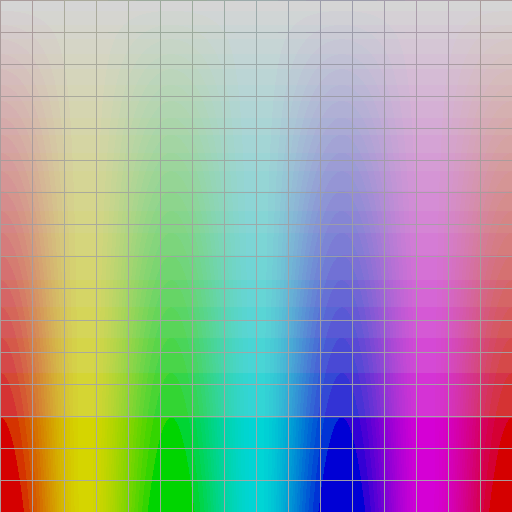
\includegraphics[width=\linewidth]{img/uplifting_texture_copyNeighbor.png}
		\caption{Nearest\\Neighbor}
		\label{fig:sigUpliftNearestNeighbor}
	\end{subfigure} \hspace{0.05em}
	\begin{subfigure}[t]{0.22\textwidth}
		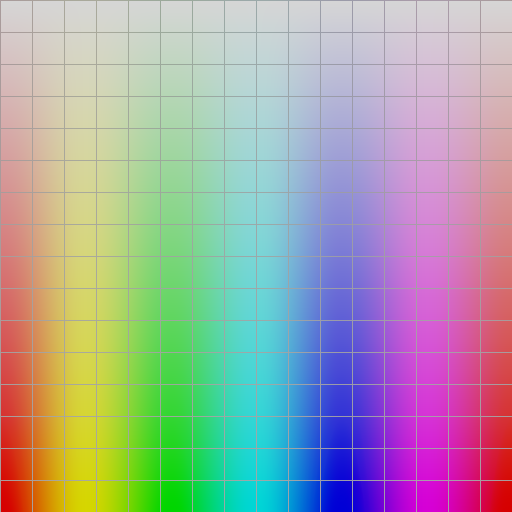
\includegraphics[width=\linewidth]{img/uplifting_texture_interpCoeff.png}
		\caption{Interpolated\\Coefficients}
		\label{fig:sigUpliftInterpCoeff}
	\end{subfigure} \hspace{0.05em}
	\begin{subfigure}[t]{0.22\textwidth}
		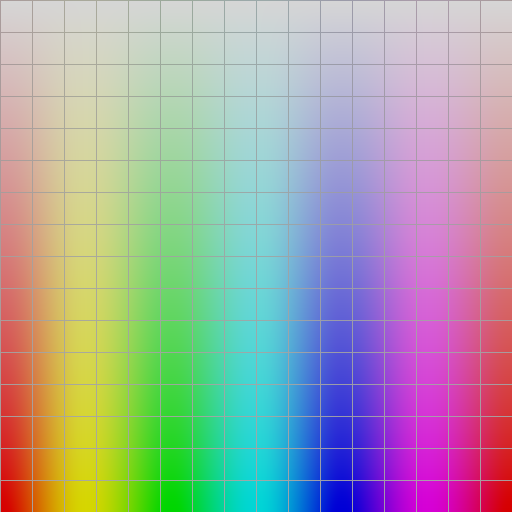
\includegraphics[width=\linewidth]{img/uplifting_texture_interpSpectra.png}
		\caption{Interpolated\\Spectra}
		\label{fig:sigUpliftInterpSpectra}
	\end{subfigure}
	\vspace{0.5em}\\
	\begin{subfigure}[t]{0.22\textwidth}
		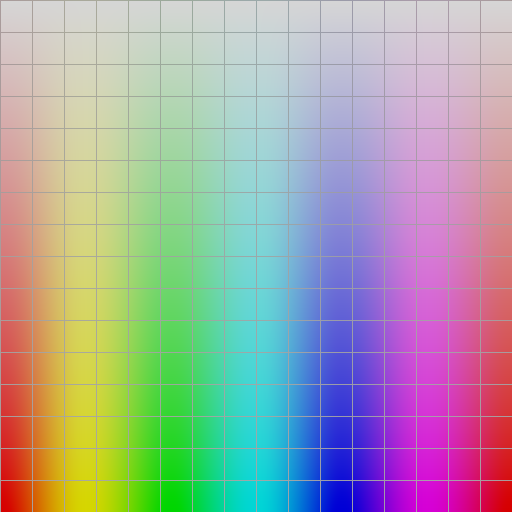
\includegraphics[width=\linewidth]{img/uplifting_texture_original.png}
		\caption{Original\\ }
		\label{fig:sigUpliftOriginal}
	\end{subfigure} \hspace{0.05em}
	\begin{subfigure}[t]{0.22\textwidth}
		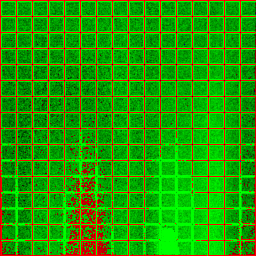
\includegraphics[width=\linewidth]{img/uplifting_diff_originalNeighbor.png}
		\caption{Original\\vs\\Nearest Neighbor}
		\label{fig:sigDiffOrigNeighbor}
	\end{subfigure} \hspace{0.05em}
	\begin{subfigure}[t]{0.22\textwidth}
	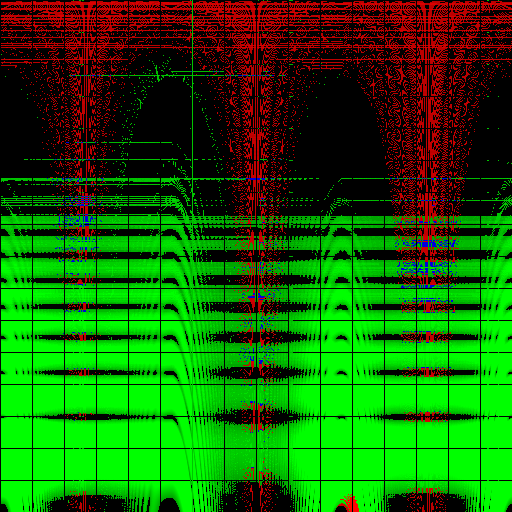
\includegraphics[width=\linewidth]{img/uplifting_diff_originalCoef.png}
	\caption{Original\\vs\\Interp. Coefficients}
	\label{fig:sigDiffSpectraCoeffs}
	\end{subfigure}\hspace{0.05em}
	\begin{subfigure}[t]{0.22\textwidth}
	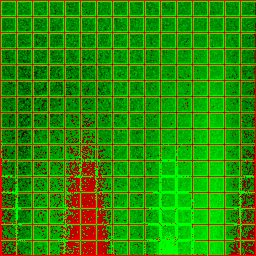
\includegraphics[width=\linewidth]{img/uplifting_diff_originalSpectra.png}
	\caption{Original\\vs\\Interp. Spectra}
	\label{fig:sigDiffOrigSpectra}
	\end{subfigure}
	\caption{Comparison of techniques for obtaining spectra for non-mapped RGB triplets in the RGB cube as created by Borgtool. The exposure of the difference images ( e), f) and h) ) is increased to 10 for the errors to be visible.}
	\label{fig:sigmoidTexture}
\end{figure}

An obvious case in which it is possible to avoid any kind of interpolation or approximation is when the RGB values that will be required during the uplift are known beforehand. They can then be added as lattice points to the RGB cube. This is especially useful when attempting to uplift specific textures or materials, which is, in fact, what this method was originally intended for.

This uplifting model is, in many cases, superior to the ones already mentioned above. First of all, the round trip error yields 0 in the sRGB gamut. In other gamuts within the spectral locus, it outperforms other models as well. Moreover, the execution speed is by far the best, even with the uplifting process running beforehand. 

The smoothness of the spectra can be considered both an advantage and a limitation. Although such spectra closely resemble real-life spectra and are suitable for the interpolation process, they cannot describe extremely bright and saturated spectra, as these tend to be more blocky.

The approach by~\citet{upsamplingFluorescence} tries to solve this issue by extending the set of three sigmoid coefficients with three additional ones specifically designed for handling fluorescence. Its goal is to avoid creating blocky spectra at gamut boundaries and rather to create smooth spectra with added fluorescent dyes to compensate for the lack of saturation. Similarly to~\citet{upsamplingJakobHanika}, the uplifting model is based on an RGB cube structure optimized by the CERES solver. As expected, the optimization takes longer, as it has 6 coefficients to consider. However, the method is the first one capable of simulating fluorescent spectra, which is especially useful for wide-gamut input textures.

The problem arising with a requirement to uplift RGB values that do not have a mapping is solved in a different manner than in the previous approach. As both the nearest neighbor and interpolation of coefficients do not produce satisfactory results, \emph{reradiation matrices} of the neighbor lattice points are used. Although this leads to higher memory requirements, the results are smoother and do not produce disruptive artifacts. 

In this section, we have presented multiple techniques capable of spectral uplifting. They differ in numerous aspects --- the round-trip error, execution time, the gamut they are capable of uplifting, whether all uplifting constraints are satisfied, etc. However, the aspect we focus on most in this thesis is the shape of the uplifted spectra, which further affects the color's behavior during rendering, especially under various illuminants. We show a comparison of spectral shapes created by different techniques by uplifting the same RGB value in~\cref{fig:upliftingTechniques}.

\begin{figure}[t!]
	\centering
	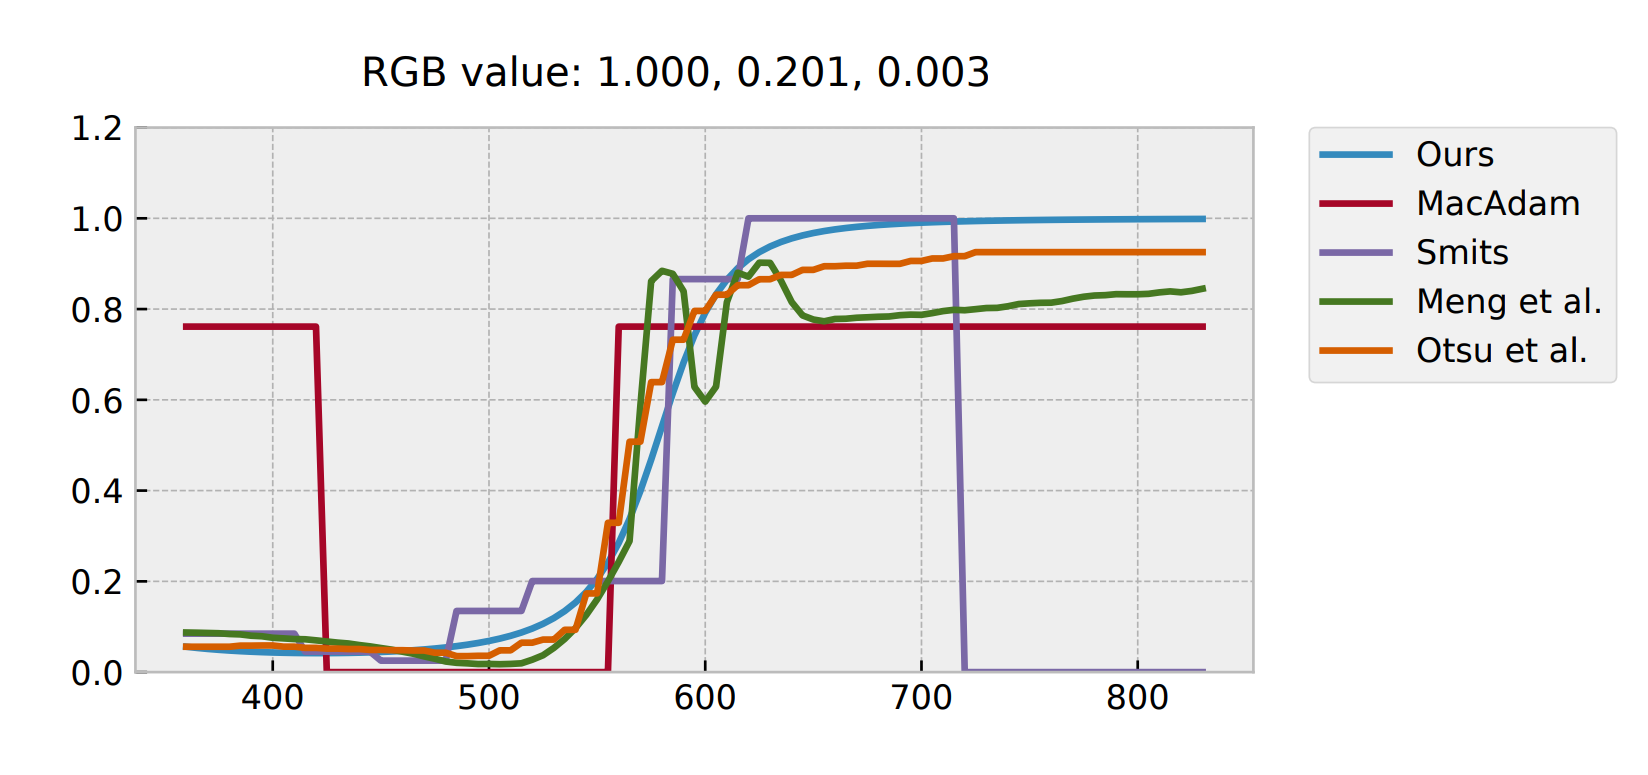
\includegraphics[width=0.8\linewidth]{img/upsampling_techniques.png}
	\caption{Comparison of spectral uplifting techniques as shown by~\citet{upsamplingJakobHanika}. All spectra were created by uplifting the (1, 0.201, 0.003) RGB value and the results were plotted according to the corresponding techniques. The ``Ours'' approach, in this case, refers to the approach by~\citet{upsamplingJakobHanika}.}
	\label{fig:upliftingTechniques}
\end{figure}

\section{Constrained spectral uplifting}

Achieving identity of uplifted spectra to the real-world spectra is, obviously, impossible. However, uplifting many RGB-based assets does not require us to be able to uplift the whole RGB gamut, but only the spectra used for the creation of said assets. As it is pretty common for artists in the VFX modeling industry to use specific color atlases when designing textures and materials, the ability to \emph{constrain} the uplifting system with these atlas colors would be extremely useful.

In other words, the user would define specific RGB:spectra mappings which would later be used in order to uplift certain RGB triplets. RGB values that would not have a pre-defined mapping would be uplifted by altering the curves of their already-mapped neighbors. 

We call this process \emph{constrained spectral uplifting}. The fact that it does not provide as much freedom as other spectral uplifting approaches works for our benefit, as the results are not a subject to high metamerism, which is, after all, the goal of this thesis.

In this thesis, we base the algorithm used to implement constrained spectral uplifting on~\cref{alg:upliftingAlgSigmoid}. We also use an RGB cube as a structure for saving the mappings, and we also create an uplifting model before rendering. We leave the specific details of implementation to ref. In this section, we discuss the theoretical background of the constraining itself. Specifically, we focus on the means of storing the individual spectra in our structure and the problems that arise along with it.

\subsection{Spectral sampling}

The constraining process starts when the user inserts a set of spectra. Finding an RGB match and creating a mapping is a straightforward task --- one must simply convert the spectra to RGB. However, the spectra must then be stored in the structure, which requires its discretization.

As the spectra must already be discretized on the input by the user (e.g. each spectrum can be defined in a form of an array which specifies reflectance values in 1nm intervals, starting from 380nm), the first approach that comes to mind is to simply store its every ith value. However, for a good color reproduction, around 30 samples are needed for each spectrum~\cite{trigonometricMomentsPresentation}. Storing so many values is extremely memory inefficient, especially when taking into account all the other mappings that must be created later in the system.

Another issue with such storage arises during the approximation stage of the uplifting process. Trying to approximate so many values is infeasible for any optimizer. We must therefore create a more compact representation, which recreates the spectra as efficiently as possible.

Although the existing approaches to spectral uplifting, which we have reviewed in~\cref{sec:upliftingMethods}, propose ways of discretizing some spectral shapes, all of them are restricted to a concrete spectral space and therefore unable to recreate all the possible reflectance curves. We see an example of this in~\cref{fig:specRecUpliftingMethods}, where the resulting spectra of the uplifting process of multiple methods are compared to the actual measured spectrum of the real-life material.

Therefore, discretization of spectra must be approached in a different way.

The simple and smooth shape of the spectra indicate that using a lower-dimensional linear function space, such as Fourier series, could be the key to their storage. Techniques based on this observation have been studied for the storage of emission spectra~\cite{fourierRepresEmission}, and appear promising also for reflectance spectra. This method is studied in an article and subsequent presentation by~\citet{trigonometricMomentsPresentation}. As the reflectance spectra are aperiodic, it is reasonable for the Fourier basis to consist of cosine transforms only. Eventually, a truncated Fourier series is used for the reconstruction, which is computed according to the following equation:
\begin{equation} \label{truncatedFourierSeries}
  f = \sum_{i=0}^{m}c_j cos(j\varphi)
\end{equation}
where $c_j$ are the Fourier coefficients eventually stored in the lattice points of the RGB cube.

We show an example of a result obtained by this method in~\cref{fig:specRecTruncatedFourier}. Although the reconstruction is not far off, the resulting spectra do not always have a physical counterpart, as the reconstruction does not obey the (0,1) reflectance range constrain. We can observe this drawback even in our example in~\cref{fig:specRecTruncatedFourier}.

\begin{figure}[t]
	\centering
	\begin{subfigure}[t]{0.45\textwidth}
		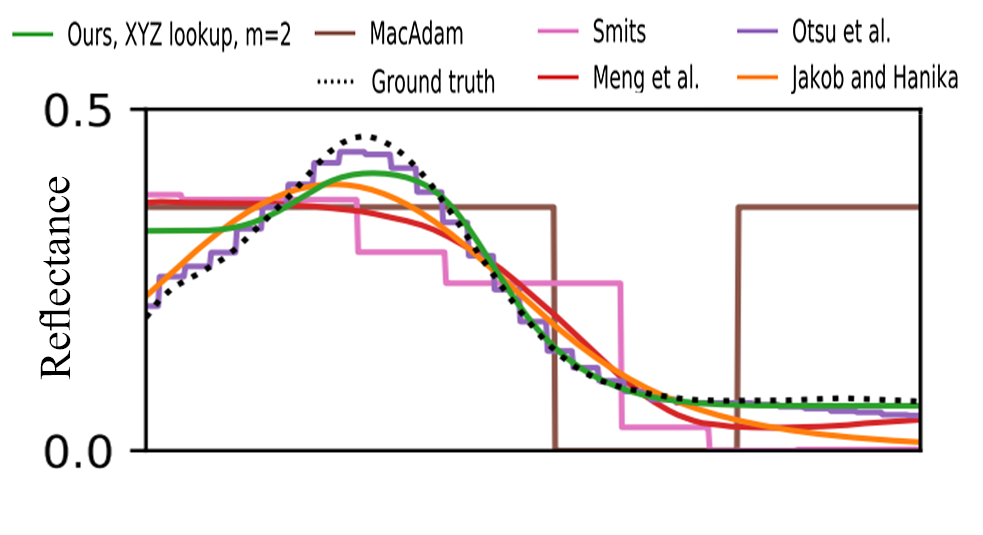
\includegraphics[width=\linewidth]{img/spectra_rec_method_comparison.png}
		\caption{Reconstruction with uplifting models as plotted by~\citet{trigonometricMomentsPaper}, where \emph{Ours} represents a newly proposed technique}
		\label{fig:specRecUpliftingMethods}
	\end{subfigure} \hspace{0.1em}
	\begin{subfigure}[t]{0.45\textwidth}
		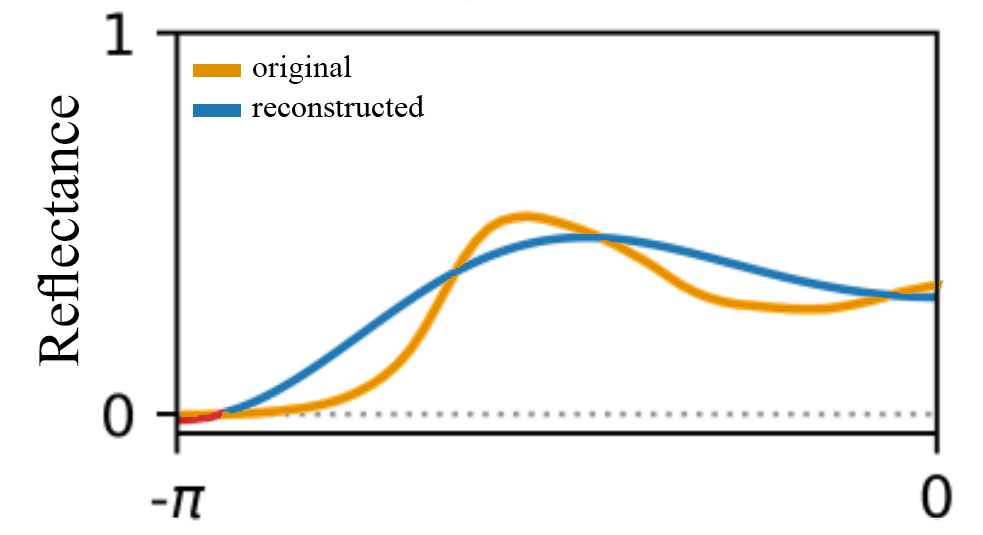
\includegraphics[width=\linewidth]{img/spectra_rec_truncated_fourier.png}
		\caption{Reconstruction with truncated Fourier series~\cite{trigonometricMomentsPresentation}}
		\label{fig:specRecTruncatedFourier}
	\end{subfigure}
	\caption{Comparison of real-life measured spectra and a few techniques that aim for reconstruction of this spectra.}
	\label{fig:spectraReconstruction}
\end{figure}

In contrast to a linear function space, spectra can also be represented non-linearly. These representations are, however, incompatible with linear prefiltering of textures~\cite{trigonometricMomentsPaper}.

To eliminate the shortcomings but utilize the strengths of both linear and non-linear methods, \citet{trigonometricMomentsPaper} propose a novel approach to spectral representation. The representation is based on the theory of moments (i.e. it is non-linear), but consists of Fourier coefficients, which implies compatibility with linear filtering. Additionally, it aims for the (0,1) range constraint satisfaction.

Following, we provide a brief overview of both the algorithm for obtaining coefficients and the reconstruction process. For more details, we refer the interested reader to the original article~\cite{trigonometricMomentsPaper}.

\paragraph{Obtaining coefficients} \label{par:spectrumToCoefficientConversion}

The first problem with obtaining the coefficients is caused by the shape of the spectra. In contrast to the Fourier basis, they are aperiodic. Their storage with Fourier coefficients therefore requires their conversion to a periodic signal.

A simple solution would be to linearly map wavelengths to a $2\pi$-periodic signal. Although such an approach can be used (we discuss its performance in ref), it causes distortions and strong artifacts at the boundaries. Moreover, Fourier coefficients computed for such signal are complex instead of real, which requires almost twice the memory for storage.

Therefore, an improvement to the mapping, called \emph{mirroring}, is proposed. It first maps the negative values of the signal as in the following equation:
\begin{equation} \label{wavelengthPhaseMapping}
\varphi =\pi \dfrac{\lambda - \lambda_{min}}{\lambda_{max} - \lambda_{min}} - \pi\in[-\pi, 0]
\end{equation}
The mapping for the positive part is then defined as the negative part mirrored, i.e. $g(\varphi) = g(-\varphi)$ for all $\varphi\in[0,\pi]$, which results in smooth transitions at the boundaries. The Fourier coefficients are then computed for this mirrored signal only and the reconstruction also uses only that part of the signal. Although this might seem wasteful, the signal created by this approach is even and therefore requires only real Fourier coefficients for its representation, which benefits the storage requirements.

Another proposed improvement to obtaining the coefficients is by focusing accuracy on important regions, also called \emph{warping}. This is achieved by means of a differentiable, bijective function that maps the wavelength range to the $[-\pi, 0]$ range and is used as a weighting function when computing coefficients. Warping of the signal is useful especially when using only a small number of coefficients, as they are unable to capture more complex curves, and it is highly recommended to always warp the signal if using less than 5 moments.

We explain our choice of the signal mapping method used for the purposes of this thesis in ref, where we also provide results of experiments that affirm our decision.

Note that using $m$ complex Fourier coefficients for storing a spectrum implies that that $m+1$ coefficients are actually saved. The $+1$ factor stands for the zeroth moment $c_0$, which is real in both the mirrored and the non-mirrored case. Therefore, overall, mirroring requires storing $m+1$ scalars, while non-mirroring requires $2m+1$ scalars.

\paragraph{Reconstruction} 

The default Fourier coefficients (without improvements such as mirroring and warping) are stored for a $2\pi$-periodic signal $d(\varphi)$, where $d(\varphi) \ge 0$ is a density for all phases $\varphi \in \R$. Therefore, they satisfy the definition of trigonometric coefficients for the \emph{trigonometric moment problem}~\cite{trigonometricMomentProblemDefiniton}. Specifically, the coefficients $\gamma$ can be expressed as
\begin{equation} \label{trigonometricCoeffsComputation}
\gamma = \int_{-\pi}^{\pi} d(\varphi) c(\varphi)d_\varphi \in C^{m+1},
\end{equation}
where $d(\varphi)$ is the finite measure that they represent, and $c(\varphi)$ is the Fourier basis.

By building upon this observation, the reconstruction of spectra is based on the theory of moments, specifically on Maximum Entropy Spectral Estimate (MESE)~\cite{unboundedMESEoriginal}. The MESE is capable of reconstructing both smooth and spiky spectra, and has been shown to produce impressive results when used for the reconstruction of emission spectra.

However, the problem with this approach is that it is not bounded, i.e. not suitable for reflectance spectra. Therefore, a novel, \emph{bounded MESE}, has been introduced. It is based on the research by~\citet{dualityBoundedUnboundedMarkoff} and, subsequently,~\citet{dualityBoundedUnboundedKrein}, who developed a duality between bounded and unbounded moment problems formulated in terms of Herglotz transform. This duality is used for transforming trigonometric moments to \emph{exponential moments} so that the bounded problem represented by the trigonometric moments has a solution if and only if the dual unbounded problem represented by the exponential moments has a solution.

The summary of the reconstruction process is as follows:
\begin{enumerate}
	\item compute exponential moments from the trigonometric moments
	\item evaluate unbounded MESE for the exponential moments
	\item compute bounded MESE by applying duality to the unbounded MESE
\end{enumerate}

We present examples of results obtained by the storage and subsequent reconstruction of reflectance spectra with the trigonometric moment method in~\cref{fig:momentsReconstructionComparison}, where we also compare the performance of different number of moments and different signal mapping techniques. For smooth spectra, even a small number of moments($m=3$) provide a quite accurate reconstruction (see~\cref{fig:momentsReconstructionPeters}). However, more complex spectra with sharper edges and spikes tend to lose detail and their reconstruction is a lot smoother. As seen in~\cref{fig:momentsReconstructionOur}, especially for the ``black'' and ``neutral35'' patches, even 7 moments are not capable of describing the original curve accurately.

Emission spectra perform even worse. To give an example, even a mirrored approach with $m=31$ is unable to reconstruct the most spiky details~\cite{trigonometricMomentsPaper}. However, as the focus of this thesis is purely on reflectance spectra, we most likely will not encounter a spectrum that would require such high number of moments.

The optimal number of moments for a spectral reflectance curve depends on many factors, such as the shape of the curve, memory limitations and the accuracy for which we aim, either in terms of curve similarity or color error under various illuminants. We discuss these factors more thoroughly as we progress with this thesis, and explain our method for determining the ``sufficient moment count'' in~\cref{ssec:initialization}.

Due to memory efficiency, smoother gradients, higher precision and multiple other reasons, thoroughly  explained in~\cref{chap:implementation}, we decide to use variable number of moments per an input reflectance spectrum. Therefore, although~\citet{trigonometricMomentsPaper} state that the interpolation of coefficients provides satisfactory results, our uplifting process cannot rely on this method for uplifting non-mapped RGB values. The only way in which to achieve this would be to reconstruct all the spectra in the corner voxels and subsequently save them with the same number of coefficients, which is not only less time efficient than interpolation of spectra, but could also result in slight discrepancies.

